\documentclass[12pt, letterpaper]{article}
\setlength{\oddsidemargin}{0.0in}
\setlength{\evensidemargin}{0.0in}
\setlength{\textwidth}{6.25in}
\setlength{\textheight}{8.5in}
\setlength{\topmargin}{-0.5in}
\usepackage{color}
\usepackage{longtable}
\usepackage{graphicx}
\usepackage{multicol}
\usepackage{cite}
\usepackage{array}
\usepackage{url}
\usepackage{amsmath}
\usepackage{amssymb}
\usepackage{algorithm}
\usepackage{subfig}
\usepackage{hhline}
\usepackage{afterpage}
\usepackage{pdflscape}
\usepackage[noend]{algpseudocode}
\usepackage{hyperref}
\usepackage[titletoc]{appendix}
\usepackage[section]{placeins}
\usepackage{float}

\usepackage{array}
\newcolumntype{L}[1]{>{\raggedright\let\newline\\\arraybackslash\hspace{0pt}}m{#1}}
\newcolumntype{C}[1]{>{\centering\let\newline\\\arraybackslash\hspace{0pt}}m{#1}}
\newcolumntype{R}[1]{>{\raggedleft\let\newline\\\arraybackslash\hspace{0pt}}m{#1}}


\makeatletter
\def\BState{\State\hskip-\ALG@thistlm}
\makeatother

\setlength\extrarowheight{2pt}
\setlength{\columnsep}{3.3cm}
\linespread{1}

\def\changemargin#1#2{\list{}{\rightmargin#2\leftmargin#1}\item[]}
\let\endchangemargin=\endlist

\renewcommand{\algorithmicrequire}{\textbf{Input:}}
\renewcommand{\algorithmicensure}{\textbf{Output:}}

\renewenvironment{abstract}
{\small
	\begin{center}
		\bfseries \abstractname\vspace{-.5em}\vspace{0pt}
	\end{center}
	\list{}{%
		\setlength{\leftmargin}{0mm}% <---------- CHANGE HERE
		\setlength{\rightmargin}{\leftmargin}%
	}%
	\item\relax}
{\endlist}


\begin{document}
	\title{\textbf{Filtering Faces\\
			\large Privacy Protection by Feature Selection \\}}
	\author{
		Artur Filipowicz\\
		\texttt{arturf@princeton.edu}\\
		Princeton University\\		
	}
	\maketitle

	
\begin{abstract} 
$\\$
This paper examines the use of filters on feature vectors for privacy protection in facial recognition. Feature vectors are the results of Fast Fourier Transform and Wavelet Transform on the Yale and Olivetti datasets. Several filters are proposed. Filters based on the signal to noise ratio and t test select feature which prevent privacy compromising reconstruction without sacrificing accuracy. The use of phase removal for FFT and normalization are also shown to protect privacy.   
\\                
\end{abstract}

\section{Introduction}
$\\$
In modern times, the existence of both terrorist threats and advance digital technology created both the need and the possibility of mass surveillance. A critical competent of such system is biometric identification of people, mainly by facial recognition. As noted in \cite{bowyer2004face}, the events of 9/11, Edward Snowden incident and other events have resulted in both a demand for recognition systems and a concern for privacy violation by such systems. While a lot of research has gone into improving facial recognition systems - \cite{bouzalmat2014comparative}, \cite{spies2000face}, \cite{bouzalmat2011facial}, 
\cite{dehai2013pca}, \cite{samra2003face} among others - relatively little research has been done on incorporating privacy into such systems; some examples being \cite{erkin2009privacy}, \cite{sadeghi2010efficient}, and \cite{kevenaar2005face}.    
\\\\
The primary approach to privacy in facial recognition is cryptography. In \cite{erkin2009privacy}, Eigenfaces recogition system is used on homomorphically encrypted data. In this first cryptographic system for facial recognition \cite{erkin2009privacy}, the client wants the server to identify a face without revealing the image to the server. 
The server also does not want to reveal the contents of it's database. In this approach, data is quantized for Pailler encryption and server and client share computations needed for matching faces. \cite{erkin2009privacy} Experimentally, 96\% accuracy was achieved in \cite{erkin2009privacy} on "ORL Database of Faces". \cite{sadeghi2010efficient} improved the algorithm presented in \cite{erkin2009privacy} by reducing the time and space complexity with the use of garbled circuits. 
\\\\
Along a different line of research, \cite{kevenaar2005face} used Helper Data Systems to provide privacy. The approach generates binary feature vector by determining reliable bits based on statistics from sample data. In the following paper, I investigate a similar approach to privacy. However, in my proposed approach no encryption or quantization is necessary. In my approach there are not additional processes. Privacy is built into the classification process. 
\\\\
This approach rests on the idea that privacy is compromised when an image can be visually inspected by an individual. Therefore, as long as the reconstruction of an image from a feature vector is not meaningful to a human, privacy has been maintained. Facial recognition systems often utilize Fast Fourier Transform (FFT) or Wavelet Transform (WT) as part of feature engineering. For example \cite{spies2000face}, \cite{bouzalmat2011facial}, 
\cite{dehai2013pca}, and \cite{samra2003face} use FFT or WT, their systems can be seen in Figure 1 and 2 and classification accuracies are provided in Figures 3 and 4. I investigate if in recognition systems like these, it is possible to alter the output of FFT or WT to reduce the quality of the reconstructed image without sacrificing accuracy of the classification.           

\begin{center}
	\begin{figure}[!htbp]
		\centering
		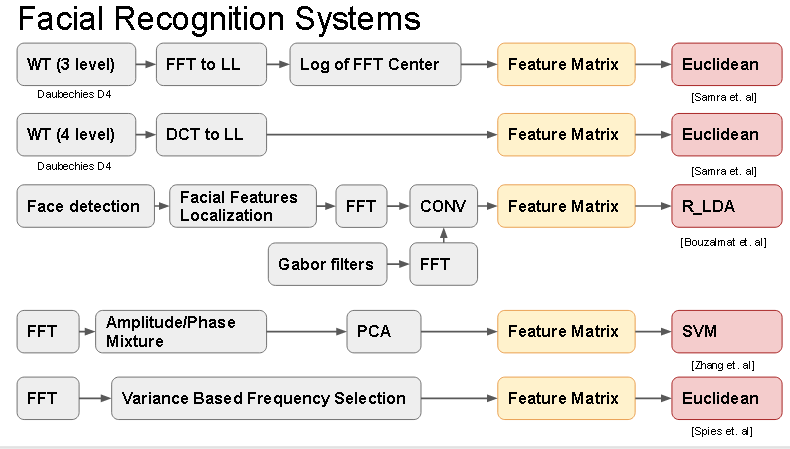
\includegraphics[width=10cm, keepaspectratio]{systems}
		\captionof{figure}{}
		\label{fig:systems}
	\end{figure}
\end{center}

\begin{center}
	\begin{figure}[!htbp]
		\centering
		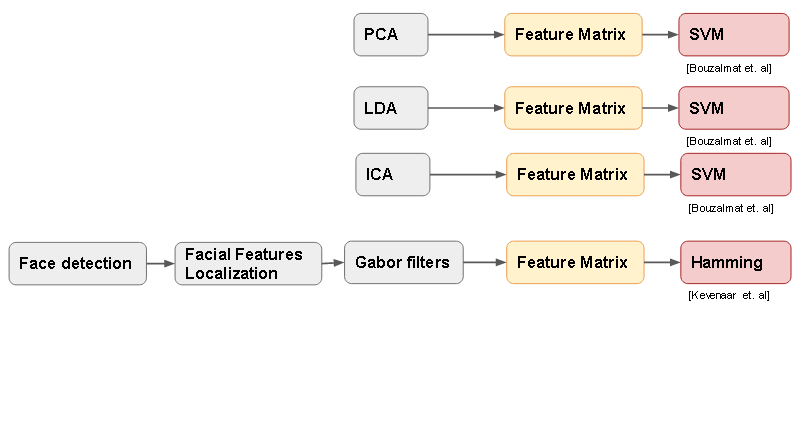
\includegraphics[width=10cm, keepaspectratio]{systems1}
		\captionof{figure}{}
		\label{fig:systems}
	\end{figure}
\end{center}

\begin{center}
	\begin{figure}[!htbp]
		\centering
		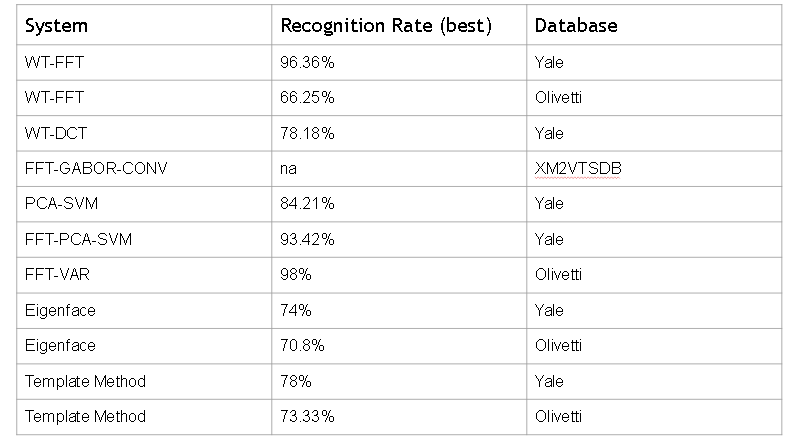
\includegraphics[width=10cm, keepaspectratio]{acc}
		\captionof{figure}{}
		\label{fig:acc}
	\end{figure}
\end{center}

\begin{center}
	\begin{figure}[!htbp]
		\centering
		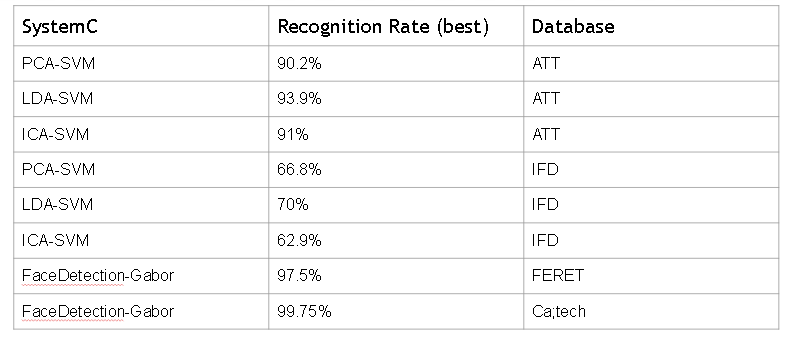
\includegraphics[width=10cm, keepaspectratio]{acc1}
		\captionof{figure}{}
		\label{fig:acc}
	\end{figure}
\end{center}

\section{My Classification Systems}

As picture in Figure 5, my classification systems for this investigation, which are very similar, begin with an application of FFT or WT to an image. Then a filter is applied as part of feature selection. Classification is accomplished with an SVM. For all of the following experiments an SVM with a leaner kernel and C = 1 was found to produce the best results.    
 
\begin{center}
	\begin{figure}[!htbp]
		\centering
		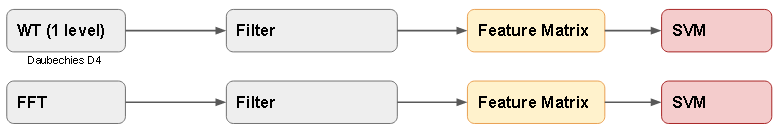
\includegraphics[width=10cm, keepaspectratio]{mysys}
		\captionof{figure}{}
		\label{fig:acc}
	\end{figure}
\end{center}

\section{Filters}

A filter is a binary matrix which selects features based on some criteria. 
Let $F_{x,d}$ be a filter $F_{x,d} \in \{0,1\}^{d x m}$ where $m$ is the number of features in each example, $x$ is one of the filter types, and $d$ is the number of features selected by the filter.
\\\\
$F_{x, d,i,j} = 1$ if $W_{x}(j)$ is with in the $d$ largest $W_{x}$, otherwise $F_{d,i,j} = 0$. 
\\\\
Let $X$ be an example: $X_{filtered} =  F_{x,d}X$
\\\\
The following Python code illustrates the mathematical definition above. In this code, 151 examples from X\_nophase are used to compute the variance of each feature, with each feature being the amplitude of a frequency from FFT. Then the 100 features with the highest 
variance are selected to pass thought the filter. 
    
\begin{verbatim}
def varFilter(train_X, numFeatures):
    F = np.zeros(train_X.shape[0])
    var = np.var(train_X, axis=1)
    varSorted = np.argsort(var)[::-1]

    F[varSorted[0:numFeatures]] = 1

    return F

(X,Y) = loadYaleData() 
X_nophase = np.zeros([X.shape[0]/2, X.shape[1]]) 
for i in range(0,X.shape[1]): 
   X_nophase[:,i] = removePhase(X[:,i])[:]

F = varFilter(X_nophase[:,0:151], 100);

X_filtered = X[np.append(F, np.ones(X.shape[0]/2), axis=0) != 1]
\end{verbatim}
$\\$
Variance is only one of the several filters investigated, and the only unsupervised filter. The other filters include rectangle and triangle filters, inspired by results in \cite{spies2000face}, which are independent of the training data, and 4 supervised filters based on the signal to noise ratio, Fisher discriminant ratio, symmetric divergence and t test. The supervised filters require a labels for positive and negative classes. During training, for each individual the training examples are divided into two classes. Positive class contains the pictures of that individual and the negative class contains all other pictures. The signal to noise ratio, Fisher discriminant ratio, symmetric divergence or t test are computed based on those two classes for each feature, and the final weight for that feature is the mean of weights cross all of the individual in the training set. 
\\\\
The filters are mathematically defined below, expect for the triangle and rectangle filters, for which Python code was a much more succinct form of definition. For the equations below, let $\mu^{+}_{j}$, $\sigma^{+}_{j}$, and $N^{+}_{j}$ be the mean, standard deviation and number of examples for the target person and let $\mu^{-}_{j}$, $\sigma^{-}_{j}$, and $N^{-}_{j}$ be the mean, standard deviation and number of examples for all other people in the database. 

\subsection{Variance}

\begin{equation} \label{Var}
W_{VAR}(j) = \sigma^{2}_{j}
\end{equation}

\subsection{Signal to Noise Ration}

\begin{equation} \label{SNR}
W_{SNR}(j) = \overline{\dfrac{| \mu^{+}_{j} - \mu^{-}_{j} |}{\sigma^{+}_{j} + \sigma^{-}_{j}}}
\end{equation}

\subsection{Fisher Discriminant Ratio}

\begin{equation} \label{FDR}
W_{FDR}(j) = \overline{\dfrac{( \mu^{+}_{j} - \mu^{-}_{j} )^{2}}{(\sigma^{+}_{j})^{2} + (\sigma^{-}_{j})^{2}}}
\end{equation}

\subsection{Symmetric Divergence}

\begin{equation} \label{SD}
W_{SD}(j) = \overline{\dfrac{1}{2} \dfrac{(\mu^{+}_{j})^{2}}{(\mu^{-}_{j})^{2}} + \dfrac{(\mu^{-}_{j})^{2}}{(\mu^{+}_{j})^{2}} + \dfrac{1}{2} \dfrac{( \mu^{+}_{j} - \mu^{-}_{j} )^{2}}{(\sigma^{+}_{j})^{2} + (\sigma^{-}_{j})^{2}} - 1}
\end{equation}

\subsection{T}

\begin{equation} \label{T}
W_{T}(j) = \overline{\dfrac{ \mu^{+}_{j} - \mu^{-}_{j}}{\sqrt{\dfrac{(\sigma^{+}_{j})^{2}}{N^{+}_{j}} + \dfrac{(\sigma^{-}_{j})^{2}}{N^{-}_{j}}}}}
\end{equation}

\subsection{Rectangle}

\begin{verbatim}
def recFilter(w,h,fw,fh):
    h = h + 1
    F = np.zeros((h,w));
    for i in range((w-1)/2+1 - fw/2, (w-1)/2+1 + fw/2 - 1):
        for j in range(h - fh - 1, h):
            F[j,i] = 1
    return np.reshape(F,(w*h),order='F')
\end{verbatim}

\begin{center}
	\begin{figure}[!htbp]
		\centering
		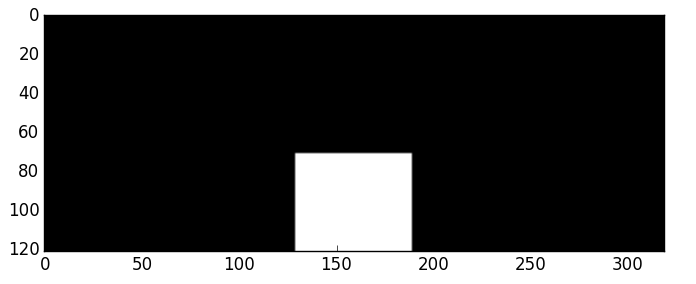
\includegraphics[width=10cm, keepaspectratio]{filters/rect}
		\captionof{figure}{Picture of a rectangle filter. White corresponds to 1.}
		\label{fig:rect}
	\end{figure}
\end{center}

\subsection{Triangle}

\begin{verbatim}
def triFilter(w,h,fw,fh):
    h = h + 1
    F = np.zeros((h,w));
    for j in range(h - fh -1, h):
        span = (j - (h - fh)) * (fw/2)/fh;
        for i in range((w-1)/2+1 - span, (w-1)/2+1 + span - 1):
            F[j,i] = 1
    return np.reshape(F,(w*h),order='F')
\end{verbatim}

\begin{center}
	\begin{figure}[!htbp]
		\centering
		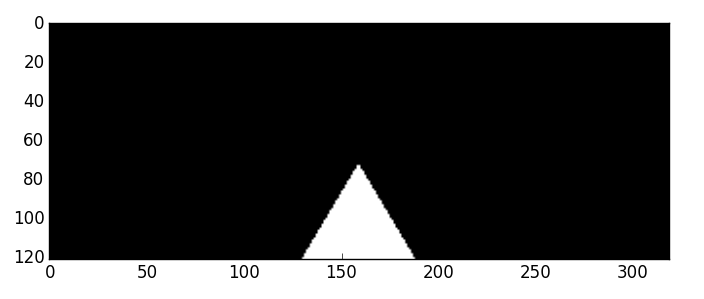
\includegraphics[width=10cm, keepaspectratio]{filters/tri}
		\captionof{figure}{Picture of a triangle filter. White corresponds to 1.}
		\label{fig:tri}
	\end{figure}
\end{center}


\section{Method}

\subsection{Classification}

Ten fold cross validation was used to test classification accuracies. Grid Search was used to optimize the SVM parameters for each fold. For all of the following experiments an SVM with a leaner kernel and C = 1 was found to produce the best results. 100 cross validations were performed and the training of supervised and unsupervised filters was constrained to appropriate fold. Since the rectangle and triangle filters are parameterized they were used to determine d for all other filters. For FFT, the filters where only applied to the amplitudes of frequencies. For WT, the filters were applied to all four maps.     

\subsection{Reconstruction}

To reconstruct original images from filtered feature vectors I set the values of all parameters which were filtered out to be zero.  

\clearpage

\section{Experimental Results}

The baseline accuracy for Yale with FFT transform is 0.741 and 0.735 when the phase is removed. The baseline for Olivetti with FFT transform is 0.975 and 0.9737 with the phase removed. The baseline for Yale with WT transform is 0.807. The baseline for Olivetti with WT transform is 0.963.    

\subsection{Basic Observations}

FFT produces a amplitude and phase for the transformed image. If the phase is removed and the image is reconstructed based on the amplitude the result is a faceless image. The image on the left is of the original, while the image on the right is the reconstruction.   

\begin{tabular}{ l r }
	\centering
	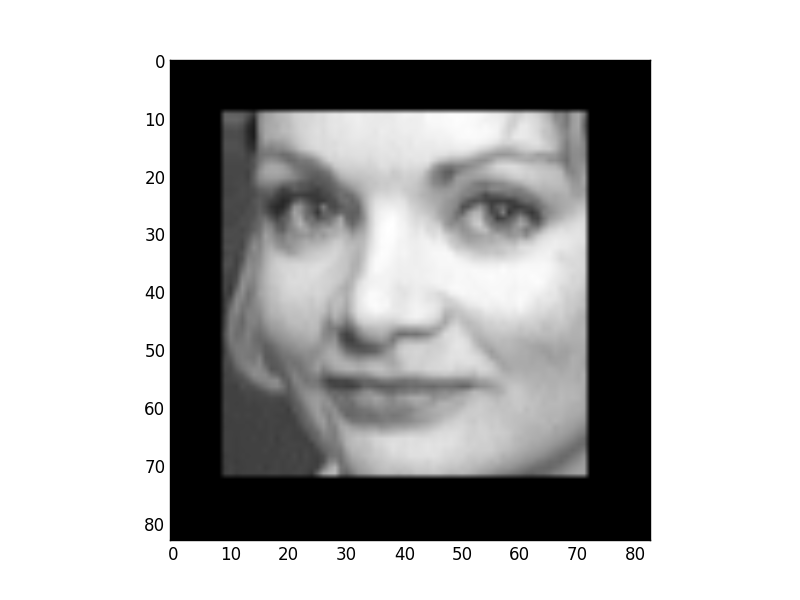
\includegraphics[width=7cm, keepaspectratio]{recon/Original1o}
	& 
	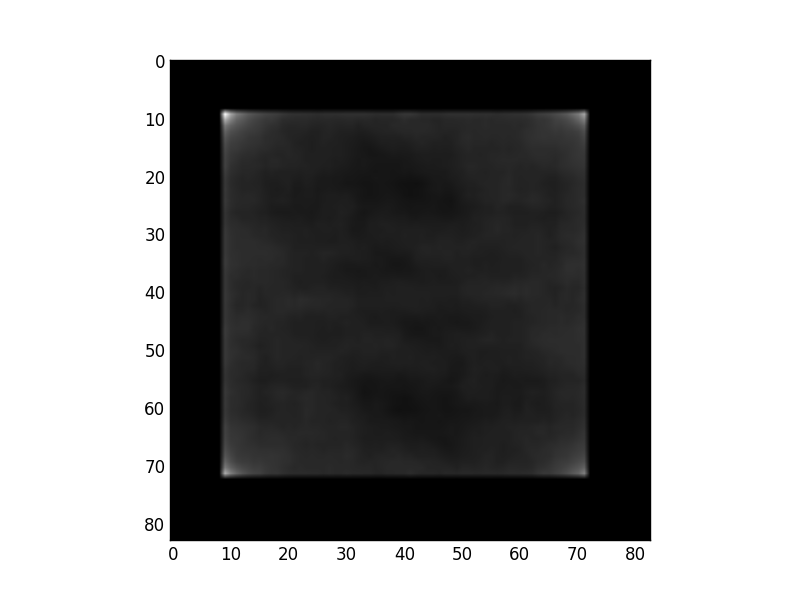
\includegraphics[width=7cm, keepaspectratio]{recon/Recon1o}
	\\
\end{tabular}

$\\$
A similar phenomena happens when the result of FFT is normalize to zero mean and unit 
variance. Top images are the spectrum and reconstruction of a normalized FFT output. The bottom images show the spectrum and reconstruction for the same image with the original mean and variance restored.    

\begin{figure}
	\centering
\begin{tabular}{ l r }
	\centering
	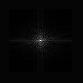
\includegraphics[width=4cm, keepaspectratio]{norm_Yale_FFT}
	& 
	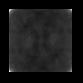
\includegraphics[width=4cm, keepaspectratio]{norm_Yale}
	\\
\end{tabular}
\end{figure}

\begin{figure}
	\centering
\begin{tabular}{ l r }
	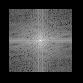
\includegraphics[width=4cm, keepaspectratio]{denorm_Yale_FFT}
	& 
	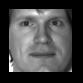
\includegraphics[width=4cm, keepaspectratio]{denorm_Yale}
	\\
\end{tabular}
\end{figure}

\clearpage

\subsection{Yale Database FFT Accuracy}

\begin{table}[H]
\centerline{\bfseries Mean Accuracy for Filters on Yale with Phase} 
\begin{tabular}{ | L{1.8cm} || R{1.8cm} | R{1.8cm}| R{1.8cm}| R{1.8cm}| R{1.8cm}| R{1.8cm}| }
	\hline
	&   \multicolumn{6}{c|}{Dimensions}   \\
	\hline
	Filter & 2115 &  2224 &  2415 &  2614 &  2915 &  3072 \\
	\hline
	Rect & 0.689 & 0.725 & 0.737   &  0.738  &  0.741  &  0.741\\
	\hline
	Var & \textbf{0.724} &  \textbf{0.728} &  0.739 &  0.741 &  0.743 &  0.743\\
	\hline
	SNR & 0.681  &  0.720 &  0.739   &    0.747  &     0.748 &  0.746\\
	\hline
	FDR & 0.687  &     \textbf{0.728} &  0.735  &     0.744  &     0.748   &    0.745\\
	\hline
	SD & 0.585 & 0.649 & 0.686 &  0.711 &  0.729 & 0.737\\
	\hline
	T & 0.685 &  0.718 &  \textbf{0.741} &  \textbf{0.749}   &    \textbf{0.750}   &     \textbf{0.747} \\
	\hline
\end{tabular}
\captionof{table}{Mean accuracy for filters on Yale with phase based on 100, 10 fold cross validations. The standard deviation for each measurement is about .07.}
\label{fig:fyp}
\end{table}

\begin{table}[H]
	\centerline{\bfseries Mean Accuracy for Filters on Yale with Phase (Triangle Filter)} 
	\begin{tabular}{ | L{1.8cm} || R{1.8cm} | R{1.8cm}| R{1.8cm}| R{1.8cm}| R{1.8cm}| R{1.8cm}| }
		\hline
		&   \multicolumn{6}{c|}{Dimensions}   \\
		\hline
		Filter & 2048 &  2088 &  2178 &  2258 &  2408 &  2528  \\
		\hline
		Tri & \textbf{0.676} &  0.713 &  \textbf{0.732} &  0.732 &  0.736   &    0.74\\
		\hline
		Var & 0.658 &  \textbf{0.726}  &     0.727 & \textbf{0.733} &  0.739   &    0.740\\
		\hline
		SNR & 0.485  &     0.657   &    0.706 & 0.719 &  0.739 & 0.743\\
		\hline
		FDR & 0.512 &  0.657 &   0.722 &  0.730 & 0.734    &   0.740\\
		\hline
		SD & 0.478 &   0.547   &    0.624 & 0.663 & 0.689 &  0.694\\
		\hline
		T & 0.487  &     0.654 & 0.707    &   0.725  &     \textbf{0.740}   &     \textbf{0.744} \\
		\hline
	\end{tabular}
	\captionof{table}{Mean accuracy for filters on Yale with phase based on 100, 10 fold cross validations. The standard deviation for each measurement is about .07.}
	\label{fig:fypt}
\end{table}

\begin{table}[H]
	\centerline{\bfseries Mean Accuracy for Filters on Yale without Phase} 
	\begin{tabular}{ | L{1.8cm} || R{1.8cm} | R{1.8cm}| R{1.8cm}| R{1.8cm}| R{1.8cm}| R{1.8cm}| }
		\hline
		&   \multicolumn{6}{c|}{Dimensions}   \\
		\hline
		Filter & 99 &  208 &   399 &   598 &   899 &  1056 \\
		\hline
		Rect & 0.689 &  0.725 &  0.737  &     0.738    &   0.741  &     0.741\\
		\hline
		Var & \textbf{0.724}  &     \textbf{0.728} &  0.739 &  0.741 &  0.743 &  0.743\\
		\hline
		SNR & 0.681   &    0.720 &  0.739 &  0.746 &  0.748 &  0.746 \\
		\hline
		FDR & 0.687   &    \textbf{0.728} &  0.735  &     0.744   &    0.748  &     0.745\\
		\hline
		SD & 0.585 &  0.649 &  0.686 &  0.711 &  0.729 &  0.737 \\
		\hline
		T & 0.685 &  0.718 & \textbf{0.741} &  \textbf{0.749}  &     \textbf{0.750}   &     \textbf{0.747} \\
		\hline
	\end{tabular}
	\captionof{table}{Mean accuracy for filters on Yale without phase based on 100, 10 fold cross validations. The standard deviation for each measurement is about .07.}
	\label{fig:fynp}
\end{table}

\begin{table}[H]
	\centerline{\bfseries Mean Accuracy for Filters on Yale without Phase (Triangle Filter)} 
	\begin{tabular}{ | L{1.8cm} || R{1.8cm} | R{1.8cm}| R{1.8cm}| R{1.8cm}| R{1.8cm}| R{1.8cm}| }
		\hline
		  &   \multicolumn{6}{c|}{Dimensions}   \\
		\hline
		Filter & 32 &   72 &  162 &  242 &  392 &  512  \\
		\hline
		Tri & \textbf{0.676}  & 0.713 & \textbf{0.732} & 0.732 & 0.736   &    0.74\\
		\hline
		Var & 0.658 &  \textbf{0.726}   &    0.727 &  \textbf{0.733}   &  0.739 &  0.740\\
		\hline
		SNR & 0.485   &    0.657   &    0.706 &  0.719  & 0.739 &  0.743\\
		\hline
		FDR & 0.512 &  0.657 &  0.722 &  0.731   &    0.734  &     0.740\\
		\hline
		SD & 0.478 & 0.547    &   0.624 & 0.663 & 0.689 & 0.694\\
		\hline
		T & 0.487  &     0.654 &  0.707   &    0.725   &    \textbf{0.740}   &     \textbf{0.744} \\
		\hline
	\end{tabular}
	\captionof{table}{Mean accuracy for filters on Yale without phase based on 100, 10 fold cross validations. The standard deviation for each measurement is about .07.}
	\label{fig:fynpt}
\end{table}



\subsection{Olivetti Database FFT Accuracy}

\begin{table}[H]
	\centerline{\bfseries Mean Accuracy for Filters with Phase Olivetti } 
	\begin{tabular}{ | L{1.8cm} || R{1.8cm} | R{1.8cm}| R{1.8cm}| R{1.8cm}| R{1.8cm}| R{1.8cm}| }
		\hline
		&   \multicolumn{6}{c|}{Dimensions}   \\
		\hline
		Filter & 2115 &  2224 &  2415 &  2614 &  2915 &  3072 \\
		\hline
		Rect & \textbf{0.971} &   \textbf{0.967} &  0.967 &  0.967 &  \textbf{0.968} & 0.967\\
		\hline
		Var & 0.968  &  \textbf{0.967} &  \textbf{0.970}  &   0.967 &  \textbf{0.968} & \textbf{0.969}\\
		\hline
		SNR & 0.968 & \textbf{0.967} &  0.968  &  \textbf{0.968} &  \textbf{0.968} &   0.968 \\
		\hline
		FDR & 0.967 & 0.966 &  0.965 &  0.965 &  \textbf{0.968}  &  0.968 \\
		\hline
		SD & 0.898 &  0.936 &  0.952 &  0.962 &   \textbf{0.968} & 0.967 \\
		\hline
		T & 0.967 & 0.966 & 0.968 &  0.967 &   \textbf{0.968}  &  0.968 \\
		\hline
	\end{tabular}
	\captionof{table}{Mean accuracy for filters on Olivetti with phase based on 100, 10 fold cross validations. The standard deviation for each measurement is about .03.}
	\label{fig:fop}
\end{table}

\begin{table}[H]
	\centerline{\bfseries Mean Accuracy for Filters on Olivetti with Phase (Triangle Filter)} 
	\begin{tabular}{ | L{1.8cm} || R{1.8cm} | R{1.8cm}| R{1.8cm}| R{1.8cm}| R{1.8cm}| R{1.8cm}| }
		\hline
		&   \multicolumn{6}{c|}{Dimensions}   \\
		\hline
		Filter & 2048 &  2088 &  2178 &  2258 &  2408 &  2528  \\
		\hline
		Tri & \textbf{0.964}  &  \textbf{0.969}  &  0.968 & 0.967 &  0.967  & 0.968\\
		\hline
		Var & 0.959  &  0.968  & \textbf{0.969} &  \textbf{0.968} &   \textbf{0.970}  &   \textbf{0.969}\\
		\hline
		SNR & 0.936&  0.964  &  0.966 &  0.967 &   0.968 &   0.968\\
		\hline
		FDR &  0.943 & 0.967 & 0.967  &  0.966 &   0.965 &  0.965\\
		\hline
		SD & 0.812 & 0.873 & 0.930   &  0.940 & 0.952 & 0.961\\
		\hline
		T & 0.932 & 0.966 & 0.967 & 0.967 & 0.968 & 0.967  \\
		\hline
	\end{tabular}
	\captionof{table}{Mean accuracy for filters on Olivetti with phase based on 100, 10 fold cross validations. The standard deviation for each measurement is about .03.}
	\label{fig:fopt}
\end{table}

\begin{table}[H]
	\centerline{\bfseries Mean Accuracy for Filters on Olivetti without Phase } 
	\begin{tabular}{ | L{1.8cm} || R{1.8cm} | R{1.8cm}| R{1.8cm}| R{1.8cm}| R{1.8cm}| R{1.8cm}| }
		\hline
		&   \multicolumn{6}{c|}{Dimensions}   \\
		\hline
		Filter & 99 &  208 &   399 &   598 &   899 &  1056 \\
		\hline
		Rect & 0.971  &  0.967 &  \textbf{0.967} &  0.967 &  \textbf{0.968} & 0.967\\
		\hline
		Var & \textbf{0.968}  &  \textbf{0.967} & \textbf{0.970}  &   0.967 &  \textbf{0.968} &  \textbf{0.969}\\
		\hline
		SNR & \textbf{0.968} & \textbf{0.967} & 0.968  &  \textbf{0.969}  & \textbf{0.968} &   0.968 \\
		\hline
		FDR & 0.967 & 0.966 & 0.965 &  0.965 & \textbf{0.968} &   0.968\\
		\hline
		SD & 0.898 &  0.936 & 0.952 &  0.962  &  \textbf{0.968} & 0.967 \\
		\hline
		T & 0.967 & 0.966 & 0.968 & 0.966 & \textbf{0.968} &   0.968 \\
		\hline
	\end{tabular}
	\captionof{table}{Mean accuracy for filters on Olivetti without phase based on 100, 10 fold cross validations. The standard deviation for each measurement is about .03.}
	\label{fig:foop}
\end{table}

\begin{table}[H]
	\centerline{\bfseries Mean Accuracy for Filters on Olivetti without Phase (Triangle Filter)} 
	\begin{tabular}{ | L{1.8cm} || R{1.8cm} | R{1.8cm}| R{1.8cm}| R{1.8cm}| R{1.8cm}| R{1.8cm}| }
		\hline
		&   \multicolumn{6}{c|}{Dimensions}   \\
		\hline
		Filter & 32 &   72 &  162 &  242 &  392 &  512  \\
		\hline
		Tri & \textbf{0.964} &   \textbf{0.969}  &  0.968 & 0.967 &  0.967 &  0.968\\
		\hline
		Var & 0.959  &  0.968 &  \textbf{0.969} &  \textbf{0.968}  &  \textbf{0.970} &    \textbf{0.969}\\
		\hline
		SNR & 0.936  &  0.964  &  0.966 & 0.967  &  0.968 &   0.968\\
		\hline
		FDR & 0.943 & 0.967 & 0.967  &  0.966  &  0.965 &  0.965\\
		\hline
		SD & 0.812 & 0.873 & 0.930  &   0.940 & 0.952&   0.961\\
		\hline
		T & 0.932  &  0.966 &  0.967 & 0.967&  0.968 & 0.967  \\
		\hline
	\end{tabular}
	\captionof{table}{Mean accuracy for filters on Olivetti without phase based on 100, 10 fold cross validations. The standard deviation for each measurement is about .03.}
	\label{fig:foopt}
\end{table}

\subsection{Yale Database WT Accuracy}

\begin{table}[H]
	\centerline{\bfseries Mean Accuracy for Filters on Yale with Wavelette} 
	\begin{tabular}{ | L{1.8cm} || R{1.8cm} | R{1.8cm}| R{1.8cm}| R{1.8cm}| R{1.8cm}| R{1.8cm}| }
		\hline
		&   \multicolumn{6}{c|}{Dimensions}   \\
		\hline
		Filter & 99 & 208 & 399 & 598 & 899 & 1056 \\
		\hline
		Var &  0.498 & 0.647 &  0.737 & 0.782  & 0.804 & 0.800 \\
		\hline
		SNR & 0.754 &  0.791 &  \textbf{0.813}  &  \textbf{0.812} & 0.815 & 0.817\\
		\hline
		FDR & 0.758 & \textbf{0.792}  &  0.807 &  \textbf{0.812}  &   \textbf{0.823} & \textbf{0.820}\\
		\hline
		SD & 0.420 & 0.524 &  0.672 & 0.725 & 0.776 & 0.783 \\
		\hline
		T &  \textbf{0.760} & 0.783 & 0.812 & \textbf{0.812} & 0.816 & 0.816 \\
		\hline
	\end{tabular}
	\captionof{table}{Mean accuracy for filters on Yale with wavelette transform based on 100, 10 fold cross validations. The standard deviation for each measurement is about .07.}
	\label{fig:fyw}
\end{table}

\subsection{Olivetti Database WT Accuracy}

\begin{table}[H]
	\centerline{\bfseries Mean Accuracy for Filters on Olivetti with Wavelette} 
	\begin{tabular}{ | L{1.8cm} || R{1.8cm} | R{1.8cm}| R{1.8cm}| R{1.8cm}| R{1.8cm}| R{1.8cm}| }
		\hline
		&   \multicolumn{6}{c|}{Dimensions}   \\
		\hline
		Filter & 99 & 208 & 399 & 598 & 899 & 1056 \\
		\hline
		Var &  0.752 & 0.853 & 0.941  &  0.971 &  0.978 & 0.980 \\
		\hline
		SNR & 0.946 &  0.957 & 0.968 &   0.974 & 0.984 & 0.985\\
		\hline
		FDR & 0.934  &  0.959 &  0.969 & \textbf{0.978} &  \textbf{0.985} &  \textbf{0.987}\\
		\hline
		SD & 0.762 & 0.811 &  0.883 & 0.919 & 0.947 &  0.958 \\
		\hline
		T &  \textbf{0.950} &  \textbf{0.960} & 0.969  &  0.972 & 0.984 &  0.986 \\
		\hline
	\end{tabular}
	\captionof{table}{Mean accuracy for filters on Olivetti with wavelette transform based on 100, 10 fold cross validations. The standard deviation for each measurement is about .03.}
	\label{fig:fow}
\end{table}

\subsection{Yale Database FFT Accuracy Graphs}

\begin{center}
	\begin{figure}[H]
		\centering
		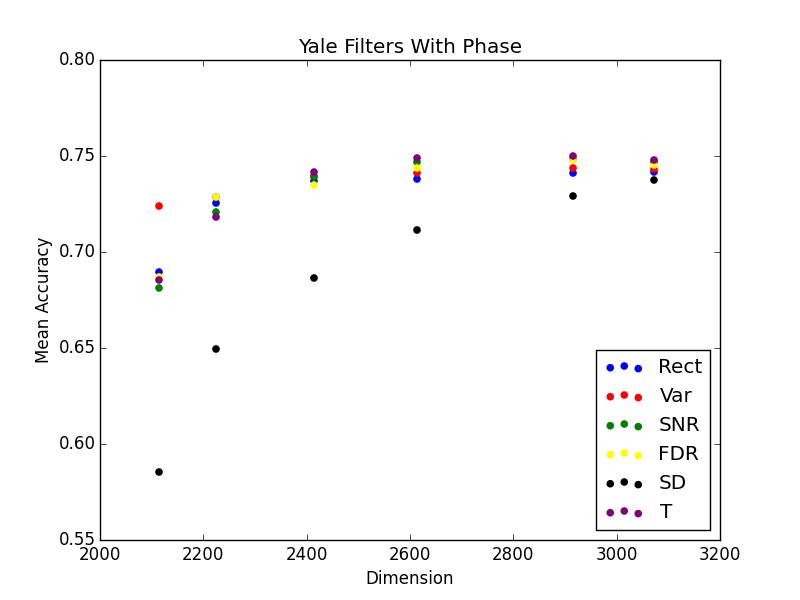
\includegraphics[width=10cm, keepaspectratio]{fftAcc/y_filters_phase}
		\captionof{figure}{}
		\label{fig:gfyp}
	\end{figure}
\end{center}

\begin{center}
	\begin{figure}[H]
		\centering
		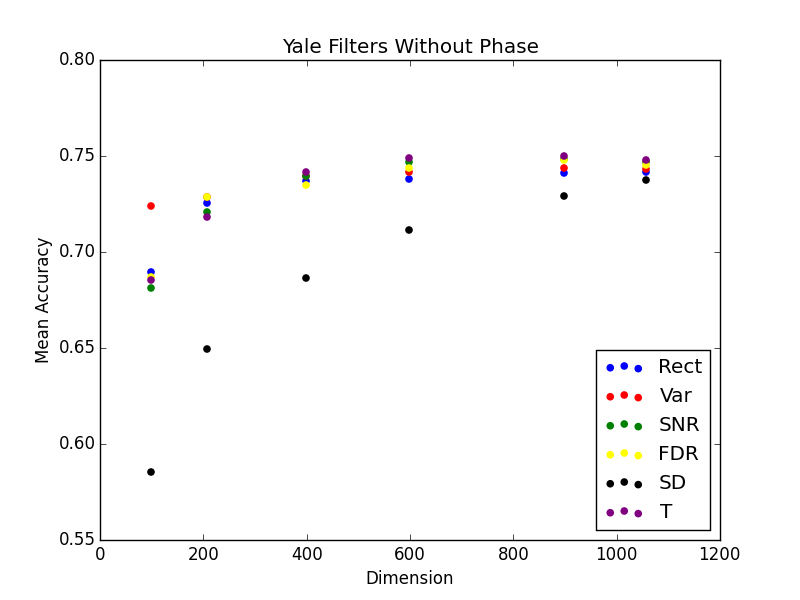
\includegraphics[width=10cm, keepaspectratio]{fftAcc/y_filters_nophase}
		\captionof{figure}{}
		\label{fig:gfyop}
	\end{figure}
\end{center}

\begin{center}
	\begin{figure}[H]
		\centering
		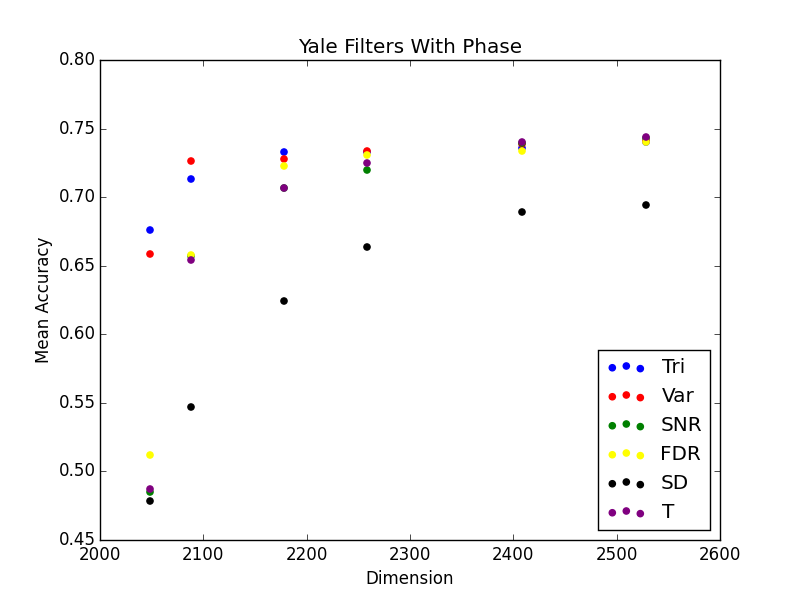
\includegraphics[width=10cm, keepaspectratio]{fftAcc/y_filters_phase_1}
		\captionof{figure}{}
		\label{fig:gfypt}
	\end{figure}
\end{center}

\begin{center}
	\begin{figure}[H]
		\centering
		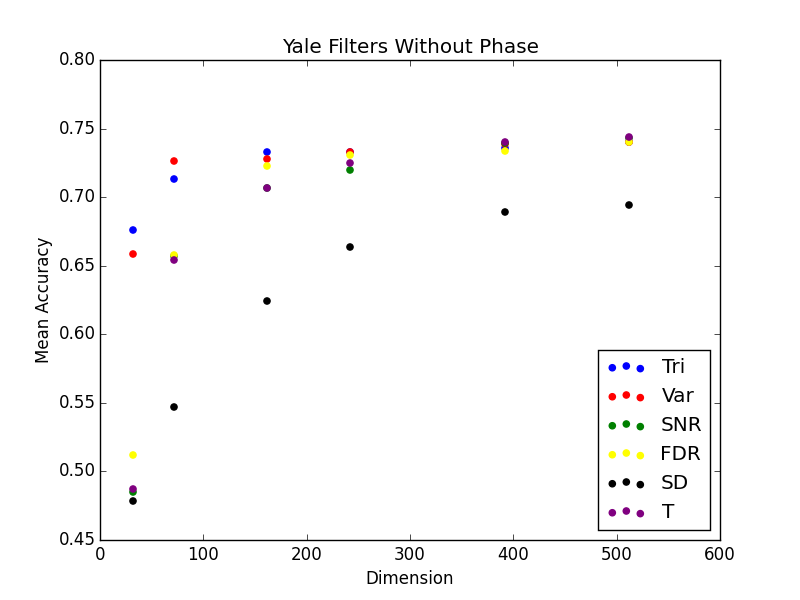
\includegraphics[width=10cm, keepaspectratio]{fftAcc/y_filters_nophase_1}
		\captionof{figure}{}
		\label{fig:gfyopt}
	\end{figure}
\end{center}

\clearpage

\subsection{Olivetti Database FFT Accuracy Graphs}

\begin{center}
	\begin{figure}[H]
		\centering
		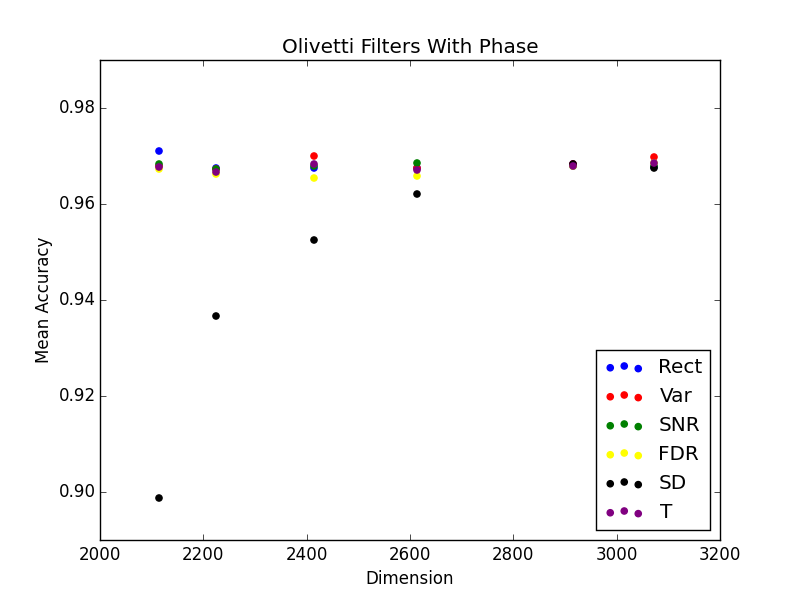
\includegraphics[width=10cm, keepaspectratio]{fftAcc/o_filters_phase}
		\captionof{figure}{}
		\label{fig:gfop}
	\end{figure}
\end{center}

\begin{center}
	\begin{figure}[H]
		\centering
		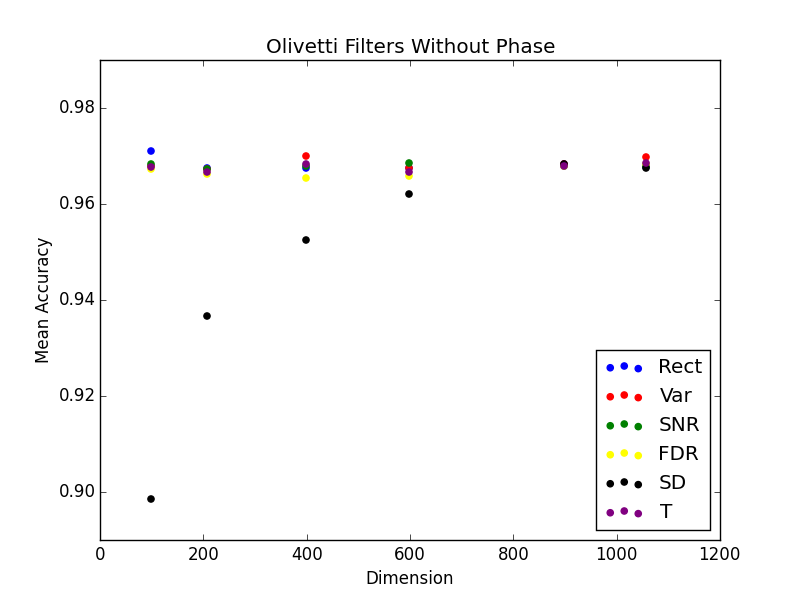
\includegraphics[width=10cm, keepaspectratio]{fftAcc/o_filters_nophase}
		\captionof{figure}{}
		\label{fig:gfoop}
	\end{figure}
\end{center}

\begin{center}
	\begin{figure}[H]
		\centering
		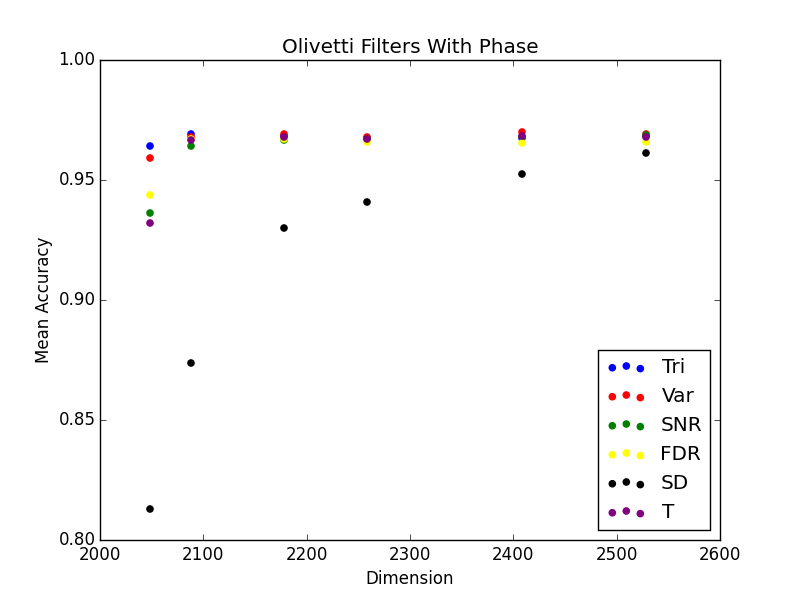
\includegraphics[width=10cm, keepaspectratio]{fftAcc/o_filters_phase_1}
		\captionof{figure}{}
		\label{fig:gfopt}
	\end{figure}
\end{center}

\begin{center}
	\begin{figure}[H]
		\centering
		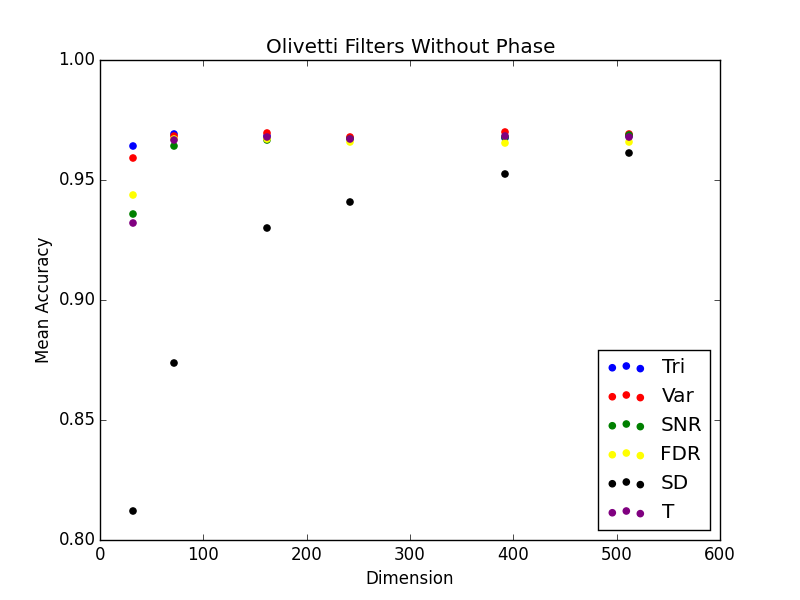
\includegraphics[width=10cm, keepaspectratio]{fftAcc/o_filters_nophase_1}
		\captionof{figure}{}
		\label{fig:gfoopt}
	\end{figure}
\end{center}

\subsection{Olivetti Database Wavelet Accuracy Graphs}

\begin{center}
	\begin{figure}[H]
		\centering
		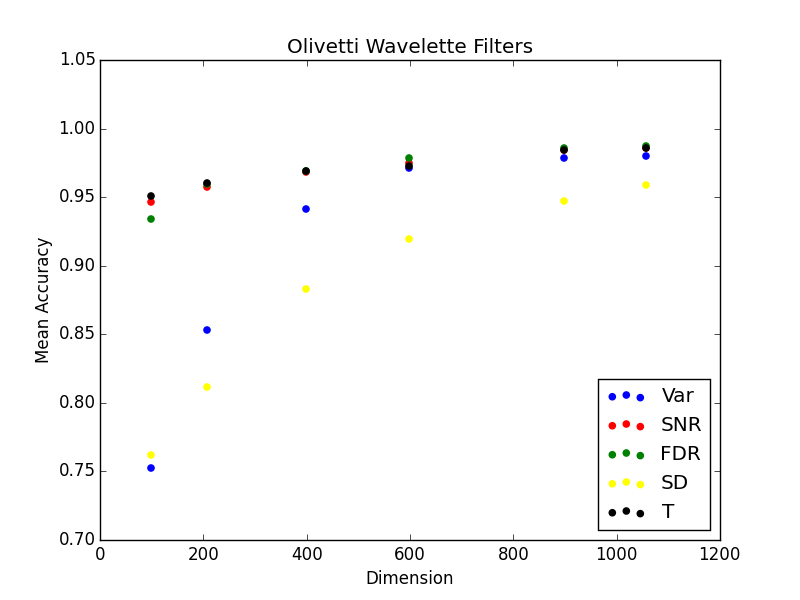
\includegraphics[width=9cm, keepaspectratio]{fftAcc/o_filters_wl}
		\captionof{figure}{}
		\label{fig:gfow}
	\end{figure}
\end{center}

\begin{center}
	\begin{figure}[H]
		\centering
		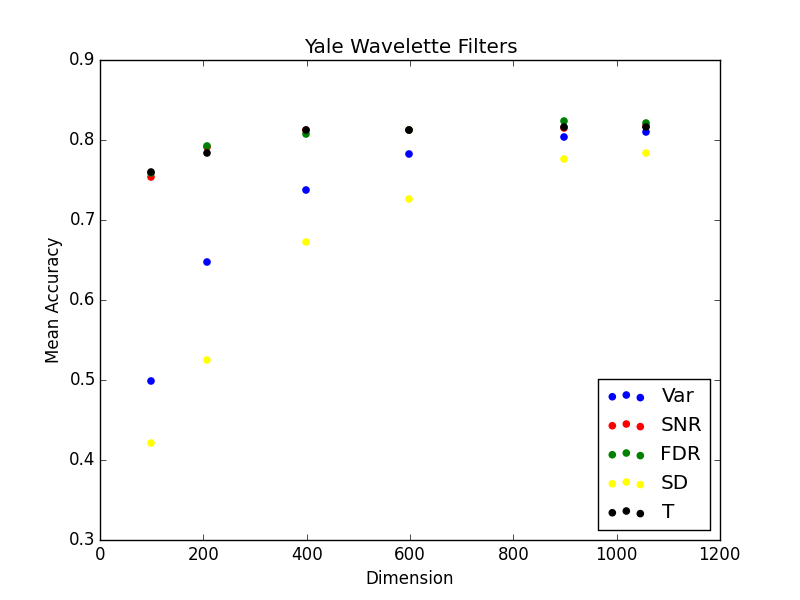
\includegraphics[width=9cm, keepaspectratio]{fftAcc/y_filters_wl}
		\captionof{figure}{}
		\label{fig:gfyw}
	\end{figure}
\end{center}

\subsection{Yale FFT Reconstructions}

\begin{table}[H]
	\begin{tabular}{cccc}
		\subfloat[Rect 99 0.68]{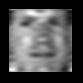
\includegraphics[width = 1.1in]{recon/rectF_99_yale}} &
		\subfloat[Rect 399 0.73]{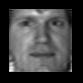
\includegraphics[width = 1.1in]{recon/rectF_399_yale}} &
		\subfloat[Rect 598 0.78]{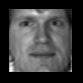
\includegraphics[width = 1.1in]{recon/rectF_598_yale}} &
		\subfloat[Rect 1056 0.74]{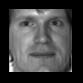
\includegraphics[width = 1.1in]{recon/rectF_1056_yale}}\\
		\subfloat[Var 99 0.724]{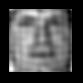
\includegraphics[width = 1.1in]{recon/varF_99_yale}} &
		\subfloat[Var 399 0.739]{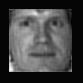
\includegraphics[width = 1.1in]{recon/varF_399_yale}} &
		\subfloat[Var 598 0.741]{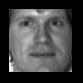
\includegraphics[width = 1.1in]{recon/varF_598_yale}} &
		\subfloat[Var 1056 0.743]{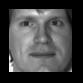
\includegraphics[width = 1.1in]{recon/varF_1056_yale}}\\
		\subfloat[SNR 99 0.681]{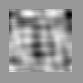
\includegraphics[width = 1.1in]{recon/snrF_99_yale}} &
		\subfloat[SNR 399 0.739]{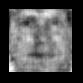
\includegraphics[width = 1.1in]{recon/snrF_399_yale}} &
		\subfloat[SNR 598 0.741]{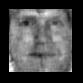
\includegraphics[width = 1.1in]{recon/snrF_598_yale}} &
		\subfloat[SNR 1056 0.74]{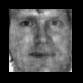
\includegraphics[width = 1.1in]{recon/snrF_1056_yale}}\\
		\subfloat[FDR 99 0.68]{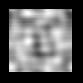
\includegraphics[width = 1.1in]{recon/fdrF_99_yale}} &
		\subfloat[FDR 399 0.73]{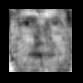
\includegraphics[width = 1.1in]{recon/fdrF_399_yale}} &
		\subfloat[FDR 598 0.74]{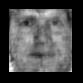
\includegraphics[width = 1.1in]{recon/fdrF_598_yale}} &
		\subfloat[FDR 1056 0.74]{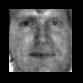
\includegraphics[width = 1.1in]{recon/fdrF_1056_yale}}\\
		\subfloat[SD 99 0.585]{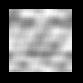
\includegraphics[width = 1.1in]{recon/sdF_99_yale}} &
		\subfloat[SD 399 0.686]{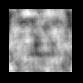
\includegraphics[width = 1.1in]{recon/sdF_399_yale}} &
		\subfloat[SD 598 0.711]{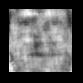
\includegraphics[width = 1.1in]{recon/sdF_598_yale}} &
		\subfloat[SD 1056 0.737]{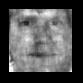
\includegraphics[width = 1.1in]{recon/sdF_1056_yale}}\\
		\subfloat[T 99 0.685]{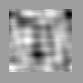
\includegraphics[width = 1.1in]{recon/tF_99_yale}} &
		\subfloat[T 399 0.741]{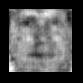
\includegraphics[width = 1.1in]{recon/tF_399_yale}} &
		\subfloat[T 598 0.749]{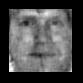
\includegraphics[width = 1.1in]{recon/tF_598_yale}} &
		\subfloat[T 1056 0.747]{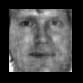
\includegraphics[width = 1.1in]{recon/tF_1056_yale}}\\
	\end{tabular}
	\caption{Reconstruction of from the filtered result of a FFT transform on the first image in the Yale database. The caption specifies filter, d, and accuracy with phase.}
	\label{hard}
\end{table}

\subsection{Yale FFT Filters}

\begin{table}[H]
	\begin{tabular}{cccc}
		\subfloat[Rect 99]{
\includegraphics[width = 1.2in]{filters/rectF_99}} &
		\subfloat[Rect 399]{
\includegraphics[width = 1.2in]{filters/rectF_399}} &
		\subfloat[Rect 598]{
\includegraphics[width = 1.2in]{filters/rectF_598}} &
		\subfloat[Rect 1056]{\includegraphics[width = 1.2in]{filters/rectF_1056}}\\
		\subfloat[Var 99]{\includegraphics[width = 1.2in]{filters/varF_99}} &
		\subfloat[Var 399]{\includegraphics[width = 1.2in]{filters/varF_399}} &
		\subfloat[Var 598]{\includegraphics[width = 1.2in]{filters/varF_598}} &
		\subfloat[Var 1056]{\includegraphics[width = 1.2in]{filters/varF_1056}}\\
		\subfloat[SNR 99]{\includegraphics[width = 1.2in]{filters/snrF_99}} &
		\subfloat[SNR 399]{\includegraphics[width = 1.2in]{filters/snrF_399}} &
		\subfloat[SNR 598]{\includegraphics[width = 1.2in]{filters/snrF_598}} &
		\subfloat[SNR 1056]{\includegraphics[width = 1.2in]{filters/snrF_1056}}\\
		\subfloat[FDR 99]{\includegraphics[width = 1.2in]{filters/fdrF_99}} &
		\subfloat[FDR 399]{\includegraphics[width = 1.2in]{filters/fdrF_399}} &
		\subfloat[FDR 598]{\includegraphics[width = 1.2in]{filters/fdrF_598}} &
		\subfloat[FDR 1056]{\includegraphics[width = 1.2in]{filters/fdrF_1056}}\\
		\subfloat[SD 99]{\includegraphics[width = 1.2in]{filters/sdF_99}} &
		\subfloat[SD 399]{\includegraphics[width = 1.2in]{filters/sdF_399}} &
		\subfloat[SD 598]{\includegraphics[width = 1.2in]{filters/sdF_598}} &
		\subfloat[SD 1056]{\includegraphics[width = 1.2in]{filters/sdF_1056}}\\
		\subfloat[T 99]{\includegraphics[width = 1.2in]{filters/tF_99}} &
		\subfloat[T 399]{\includegraphics[width = 1.2in]{filters/tF_399}} &
		\subfloat[T 598]{\includegraphics[width = 1.2in]{filters/tF_598}} &
		\subfloat[T 1056]{\includegraphics[width = 1.2in]{filters/tF_1056}}\\
	\end{tabular}
	\caption{Filters trained on Yale database. White indicated a 1. Caption specifies filter type and d.}
	\label{hard}
\end{table}

\subsection{Yale WT Reconstructions}

\begin{table}[H]
	\begin{tabular}{cccc}
		\subfloat[Var 99 0.498]{\includegraphics[width = 1.2in]{recon/varF_99_yaleWL}} &
		\subfloat[Var 399 0.737]{\includegraphics[width = 1.2in]{recon/varF_399_yaleWL}} &
		\subfloat[Var 598 0.782]{\includegraphics[width = 1.2in]{recon/varF_598_yaleWL}} &
		\subfloat[Var 1056 0.800]{\includegraphics[width = 1.2in]{recon/varF_1056_yaleWL}}\\
		\subfloat[SNR 99 0.754]{\includegraphics[width = 1.2in]{recon/snrF_99_yaleWL}} &
		\subfloat[SNR 399 0.813]{\includegraphics[width = 1.2in]{recon/snrF_399_yaleWL}} &
		\subfloat[SNR 598 0.812]{\includegraphics[width = 1.2in]{recon/snrF_598_yaleWL}} &
		\subfloat[SNR 1056 0.817]{\includegraphics[width = 1.2in]{recon/snrF_1056_yaleWL}}\\
		\subfloat[FDR 99 0.758]{\includegraphics[width = 1.2in]{recon/fdrF_99_yaleWL}} &
		\subfloat[FDR 399 0.807]{\includegraphics[width = 1.2in]{recon/fdrF_399_yaleWL}} &
		\subfloat[FDR 598 0.812]{\includegraphics[width = 1.2in]{recon/fdrF_598_yaleWL}} &
		\subfloat[FDR 1056 0.820]{\includegraphics[width = 1.2in]{recon/fdrF_1056_yaleWL}}\\
		\subfloat[SD 99 0.42]{\includegraphics[width = 1.2in]{recon/sdF_99_yaleWL}} &
		\subfloat[SD 399 0.672]{\includegraphics[width = 1.2in]{recon/sdF_399_yaleWL}} &
		\subfloat[SD 598 0.725]{\includegraphics[width = 1.2in]{recon/sdF_598_yaleWL}} &
		\subfloat[SD 1056 0.783]{\includegraphics[width = 1.2in]{recon/sdF_1056_yaleWL}}\\
		\subfloat[T 99 0.760]{\includegraphics[width = 1.2in]{recon/tF_99_yaleWL}} &
		\subfloat[T 399 0.812]{\includegraphics[width = 1.2in]{recon/tF_399_yaleWL}} &
		\subfloat[T 598 0.812]{\includegraphics[width = 1.2in]{recon/tF_598_yaleWL}} &
		\subfloat[T 1056 0.816]{\includegraphics[width = 1.2in]{recon/tF_1056_yaleWL}}\\
	\end{tabular}
	\caption{Reconstruction of from the filtered result of a wavelette transform on the first image in the Yale database. The caption specifies filter, d, and accuracy. }
	\label{hard}
\end{table}

\section{Conclusions}
$\\$
There is a lot of potential for privacy protection with proper alterations in the feature engineering process. Across all experiments the removal of the phase from the FFT result yields almost the same accuracy. However, the image becomes impossible reconstruct using simple means. Additionally, the normalization mean and variance can be hidden by the server, which also prevents reconstruction. Along the same lines, the feature vectors can be permuted by some hidden permutation matrix. 
\\\\
Regarding the filters, which should be applied even for performance improvements, SNR and T are the most useful for privacy protection. For both FFT and WT, these filters allow a large dimension reduction with almost no accuracy loss. This allows for reconstructions to be unidentifiable, see Table 11 cells j and v and Table 13 cells f and r. In general the supervised filter promote privacy in the reconstructed image. This is because they use high and low frequencies for reconstruction in FFT as seen in Table 12. The mix avoid details form being reconstructed fully. In WT, the filters prevent reconstruction of the eyes which is useful, although not fully understood. For high level of privacy, rectangle, triangle and variance filter performs best across experiments at the smallest tried d. 
\\\\
In future research consecutive search methods can be utilized to produce filters. Additionally, the reconstruction for WT should be explained in terms of the underlying bands. Lastly, a fully algorithm utilizing the filters and taking into the account the client server model should be developed.  
\\\\\\\\
This paper represents my own work in accordance with University regulations.              
\\\\\\\\

\bibliographystyle{abbrv}
\bibliography{bibl} 


\end{document}